\section{Beispiele}
 \renewcommand{\arraystretch}{2}

\begin{tabularx}{\columnwidth}{p{2.5cm} X}
	\hline 
	\multicolumn{2}{c}{\textbf{Modellbildung}}\\
	\hline 
	Fadenpendel & 
\begin{minipage}{11cm}
	$\vec{F}_G = \vec{F}_{rad} + \vec{F}_{tan}$\newline 
	nur $\vec{F}_{tan}$ berücksichtigen, da $\vec{F}_{rad}$ von 'Fadenkraft' kompensiert wird
	$\vec{F}_{tan} = -|\vec{F}_g|\cdot \sin(\varphi) = -mg \sin(\varphi)$\qquad 
	$ a(t) = \dot v(t) = l\dot \omega(t) = l\ddot \varphi(t) $
	$\vec{F}_{tan} = m \cdot a_{tan} = m\cdot l\ddot \varphi(t) = -mg\sin(\varphi) \implies$ \newline 
	$l\cdot \ddot \varphi(t) + g\sin(\varphi) = 0 \qquad \text{Taylor } \sin(\varphi) \approx \varphi$\newline  
	$l\cdot \ddot \varphi + g\cdot \varphi =0 \qquad \text{DGL lösen}$\newline 
	Ansatz: $\varphi(t) = e^{\lambda t} \qquad l\lambda^2 e^{\lambda t} + g e^{\lambda t} = 0$\newline
	$l\lambda^2 + g = 0 \qquad \lambda = \pm j\sqrt{\frac{g}{l}} \qquad \varphi(t) = A\sin\sqrt{\frac{g}{l}} + B\cos\sqrt{\frac{g}{l}}$\newline
	$\hat\varphi = \sqrt{B^2+ A^2}\qquad \varphi_0 = \frac{B}{A}\qquad \boxed{\varphi(t) = \hat \varphi\cdot \sin\left( \sqrt{\frac{g}{l}} + \varphi_0 \right)}$ 
\end{minipage}\begin{minipage}{3cm}
	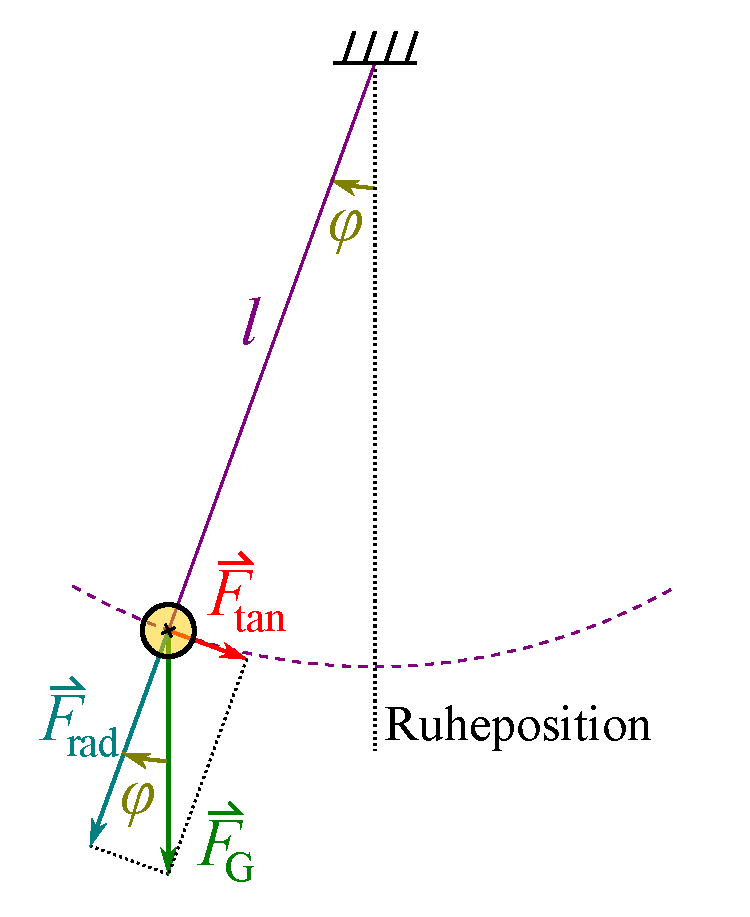
\includegraphics[width = 3cm]{images/fadenpendel}
\end{minipage}





\\		
	\hline 
	\multicolumn{2}{c}{\textbf{Gewöhliche Differentialgleichungen }}\\
	\hline 
	\multicolumn{2}{c}{1. Ordnung}\\
	\hdashline
	

Lösung durch Substitution & 
$y' = A\left(\dfrac{y}{x}\right) = A(u) \quad \text{subst.}\quad u(x) = \dfrac{y}{x} \quad u' = \dfrac{x\cdot y'-y\cdot1}{x^2} = \dfrac{y'-u}{x} $ \newline 
$y' = x\cdot u' +u = A(u)  \quad u' = \dfrac{A(u)-u}{x} \quad \text{separierbar!}$ \newline 
$\boxed{\int\dfrac{du}{A(u) - u} = \int \dfrac{dx}{x}} \quad \text{Lösung der DGL für } u(x) \quad y = x\cdot u(x)$\\
Anwendung Beispiel&
$y' = \dfrac{y}{x} - \dfrac{x^2}{y^2} \quad A(u) = u - \dfrac{1}{u^2} \quad u' = \dfrac{A(u) - u}{x} = -\dfrac{1}{u^2\cdot x} $\newline 
$-\int u^2 du = \int \dfrac{1}{x} \quad -\dfrac{u^3}{3} = ln|x|+C \quad y(x) = x \cdot u(x) = x\cdot (C -3\ln|x| )^{1/3}$
\\
	\hdashline
	\multicolumn{2}{c}{lineare DGL mit konstanten Koeffizienten}\\
	\hdashline
	Schwingungen &
ODE 2. Ordnung, konstante Koeffizienten: $m\ddot x(t) + d\dot x(t) + k x(t) = F(t)$\newline 
mech. Schwingkreis: $\ddot x(t) + 2\delta \dot x (t) + \omega_0^2 x(t) = f(t) \qquad \delta = \frac{d}{2m},\; \omega_0^2 = \frac{k}{m}\geq 0,\; f(t) = \frac{F(t)}{m}$\\

\cline{2-2}
Freie ungedämpfte Schwingung &
$f(t) =0, \delta = 0 \qquad $ 
$\ddot x(t) + \omega_0^2 x(t) = 0$\newline 
$\boxed{x(t) = C_1\cos(\omega_0 t) + C_2\sin(\omega_0 t)} \qquad \text{Eigenfrequenz}: \omega_0$ \\
\cline{2-2}
Freie gedämpfte Schwingung & 
$\delta \neq 0, f(t) = 0 \qquad $
$\ddot x(t) + 2\delta \dot x (t) + \omega_0^2 x(t) = 0 \qquad$
$x(t) = C_1 e^{\lambda_1 t} + C_2 e^{\lambda_2 t} \quad (C_1,C_2 \in \mathbb R)$\newline 
$\lambda^2 + 2\delta\lambda + \omega_0^2 = 0 \quad $
$\lambda_{1,2} = -\delta \pm \sqrt{\delta^2 -\omega_0^2} $\newline 
$\boxed{x(t) = e^{-\delta t} \left( C_1\cos\left( \sqrt{\omega_0^2 - \delta^2}\cdot t\right)  + C_2\sin\left( \sqrt{\omega_0^2 - \delta^2}\cdot t\right)  \right)}$\\
\cline{2-2}
Erzwungene Schwingung & 
$f(t) \neq 0,\quad \omega\in\mathbb{R} \quad $
Harmonische Schwingung als Anregung: $f(t) = f_0\cdot e^{j\omega t} \quad f_0>0$\newline 
$\ddot x(t) + 2\delta \dot x (t) + \omega_0^2 x(t) = f_0\cdot e^{j\omega t}\qquad $ Homogene $\mathbb{L}$ von Freier gedämpften Schwingung\newline
Ansatz: $x_p(t) = A\cdot e^{j(\omega t - \phi)}\qquad $
$-\omega^2 + 2\delta j \omega +\omega_0^2 = \dfrac{f_0}{A}e^{j\phi}$ Betrag L.H.S, Quadrieren  \newline 
$(\omega_0^2 - \omega^2)^2 + 4\delta^2\omega^2 = \dfrac{f_0^2}{A^2} \qquad $
Amplitude: $\boxed{A =  A(\omega) = \dfrac{f_0}{\sqrt{ (\omega_0^2 - \omega^2)^2 + 4\delta^2\omega^2 }}}$\newline 
$\frac{dA}{d\omega} = 0 \rightarrow \omega_{max} = \sqrt{\omega_0^2 - 2\delta^2} \quad$
$\delta = 0 \rightarrow A(\omega)\to\infty \text{ wenn } \omega \to \omega_0 $\newline
$\eta = \frac{\omega}{\omega_0} \quad$ Lehrsche Dämpfung $D=\frac{\delta}{\omega_0}$ \\


	\hline 
	\multicolumn{2}{c}{\textbf{Systeme von Differentialgleichungen}}\\
	\hline 
	\input{sections/uebungen/komplEW}
	mehrere Eigenwerte & 

$A = \begin{pmatrix} 2&1\\0&2 \end{pmatrix} \quad$
$(A-\lambda I)\bm p = 0 \quad \begin{vmatrix} 2-\lambda&1\\0&2-\lambda \end{vmatrix}=(2-\lambda)^2 = 0 \quad \lambda_{1,2} = 2$\newline
Lösungsvektor 1: $ (2-2)\cdot p_1 + 1\cdot p_2 =0\rightarrow\; \bm p_0 = (1 \;0)^t$\newline 
Lösungsvektor 2: $\bm p_1(t) = (t\bm p_0 + \bm p^*) \quad (A-\lambda I)\bm p^* = \bm p_0 \quad $
$\begin{pmatrix} 0&1\\0&0\end{pmatrix}\cdot \begin{pmatrix} p_0^1\\p_1^1\end{pmatrix} = \begin{pmatrix} 1\\0\end{pmatrix}$\newline  
$\bm p_1 = (0\; 1)^t \qquad \qquad$ 
$\bm x(t) = C_1 e^2t \begin{pmatrix} 1\\0\end{pmatrix} + C_2e^{2t} \left(t \begin{pmatrix} 1\\0\end{pmatrix} + \begin{pmatrix} 0\\1\end{pmatrix}\right) \quad (C_1,C_2\in \mathbb R)$\\
	\hline 
	\multicolumn{2}{c}{\textbf{Dynamische Systeme}}\\
	\hline
	Saddle-Node-Bifurkation &
$\dot x = r + x^2 \quad r\in\mathbb{R} \qquad f(x^*) = r+(x^*)^2 + r = 0 \implies x^*_{1,2} = \pm \sqrt{-r}$\newline 
$f'(x^*) = 2x^* = \begin{cases}> 0 & 2\cdot\sqrt{-r} \quad \text{instabile Fixpunkte}\\<0 &-2\cdot\sqrt{-r} \quad \text{stabile Fixpunkte}\end{cases}$
\\
&
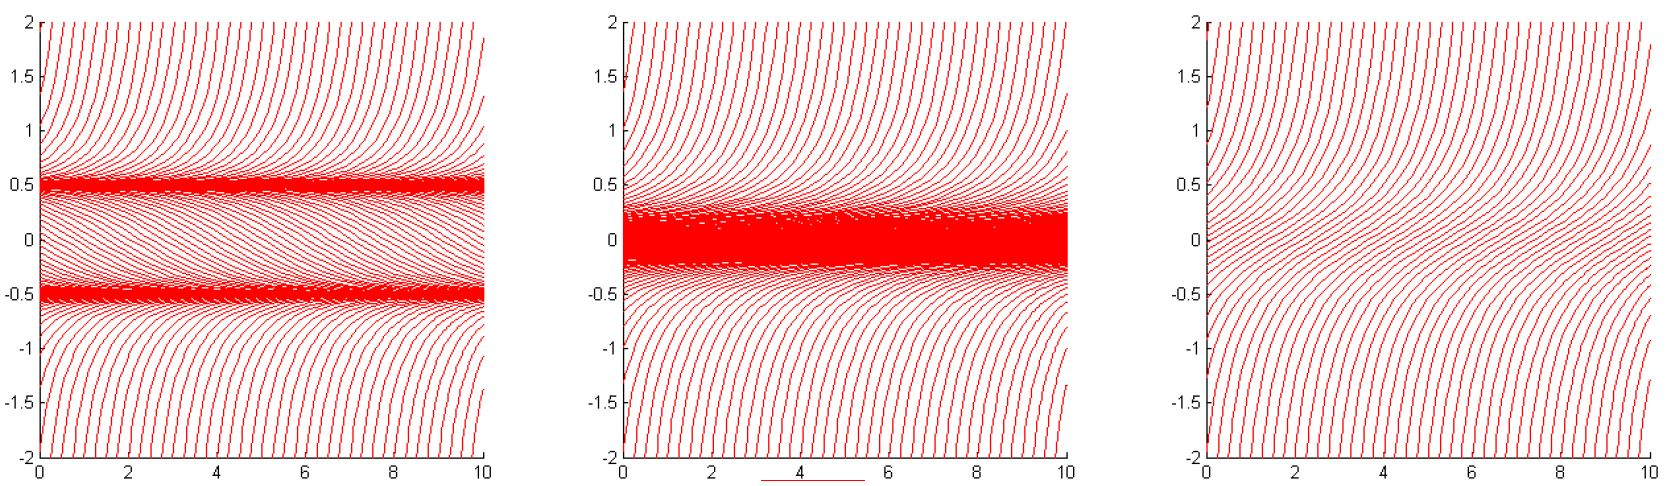
\includegraphics[scale = .15]{images/bif_saddle_node} 
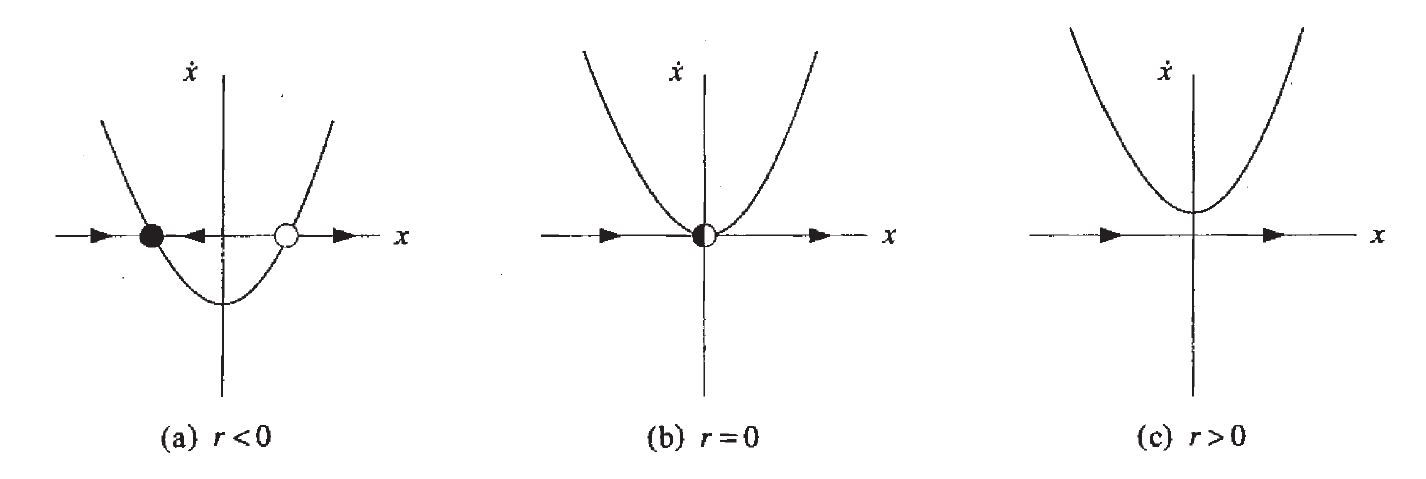
\includegraphics[scale = .15]{images/bif_saddle_node2} 
\\
	Superkritische Pitchfork-Bifurkation & $\dot x = rx-x^3 \quad  r\in\mathbb{R}$ \\
	\hdashline 
	
\end{tabularx} 



